
\documentclass{article}
\usepackage{amsmath}
\usepackage{amsfonts,amssymb}
\usepackage{pgfplots}
\usepackage{graphicx} 
\usepackage{xcolor}
\usepackage{float}
\usepackage[cache=false]{minted}
\usemintedstyle{vs}
\usepackage{listings}
\usepackage[utf8]{inputenc}
\usepackage[english]{babel}
\usepackage[
backend=biber,
style=alphabetic,
sorting=ynt
]{biblatex}


\newcommand{\norm}[1]{\| #1 \|}
\newcommand{\bignorm}[1]{\Bigl \| #1 \Bigr \| #1}
\renewcommand{\figurename}{Figure.}
\definecolor{LightGray}{gray}{0.9}
% preamble: the area before main document(序言)
% set up the value of `\maketitle`
\title{\textbf{CMT316 Applications of Machine Learning - Coursework I Part 2}}
\date{1st April, 2021}
\author{Zhiliang Xiang 2028447}
\tikzset{>=stealth}

\begin{document}
\maketitle
\pagenumbering{gobble}
\newpage
\pagenumbering{arabic}
\section*{Part 2 Report}
\paragraph{}
For the given BBC news dataset\cite{4}, we aim at building a machine learning program to classify news articles. This report will give details and justifications of each step that follows the experimental design pipeline, then show the overall performance of the model, and finally discuss how the model could be improved with respect to potential problems.
\subsection*{1. Text Preprocessing}
\paragraph{}
Starting from loading raw text document locally, once the raw data are loaded, the primary task of text preprocessing is to filter all the texts and symbols that are irrelevant to our classification task. we then conduct tokenisation and lemmatisation to the loaded data, eliminate all the stopwords and symbols from the token set. Here we only filtered some trivial symbols which commonly used in any contexts. Symbols which are related to certain contexts like '\$' or '@' won't be eliminated.
\subsection*{2. Feature Engineering} 
\paragraph{}
In this step, we extract 3 representative features:
\begin{enumerate}	
		\item  Token frequency of news contents
		\item  Token frequency of news headlines
		\item  Frequency distribution of Part of Speech Tags	
\end{enumerate}
and represent them as vectors.
\paragraph{}
We first consider a typical choice of document representation, the \textit{bags of words} approach, it could capture how much does a word contribute to the semantics of a certain document\cite{1}.
 %TODO:and transform the raw dataset into collection of vectors correspond to the chosen features. 
 We deemed the set of top frequency-ranking tokens from each topic as vocabulary, such that contents of a news can be represented as a vector, each entry of the vector records the occurrence count of a token from the vocabulary. 
\paragraph{}
 However, in the setup of raw tokens frequency, all words are considered equally important, that is, some irrelevant words that've been commonly used could be ranked to the top. In this case, we introduced the TF-IDF weighting\cite{2} scheme to apply on each token when building the vocabulary. Consider the following equation, tf$_i$ is the frequency of $i$ in topic $T$, cf$_i$ denotes the occurrences of $i$ within all topics, $n_i$ is the number of topics that contain $i$, and $N$ is the total number of topics, then the ranking score $s_i$ of token $i$ in topic $T$ is:

 \begin{equation*}
	\begin{aligned}
	s_i = \text{tf}_i * \frac{\text{tf}_i}{\text{cf}_i} * log(\frac{N}{n_i})
	\end{aligned}
\end{equation*}
By using TF-IDF weighting scheme, we can achieve that:
\begin{itemize}
	\item (High Relevance) Scores of tokens with high frequency in a certain topic will be scaled up 
	\item (Low Relevance) Scores of tokens which occurs fewer times in a topic, or occurs in many topics will be scaled down
	\item (Lowest Relevance) Scoring 0 when a token appears in all topics
\end{itemize}
\paragraph{}
By choosing the top-ranking tokens and combining sub-vocabulary from each topic, we can get the general vocabulary within all the documents. After the vocabulary was built, we iterated the each line of the documents and stored the scores into a set of arrays such that the entries represent the frequencies of top-ranking tokens in the vocabulary.
\paragraph{}
In addition, considered the news headlines could contain key information of which topic the news belongs to, for example tech news headlines usually contain 'computer' or other topic related keywords, in that case one can easily tell which topic the news is by only looking at the headline. To implement this, we separately built a top-frequency ranked vocabulary of news titles, followed the same manner as in processing news contents.
\paragraph{}
% TODO be more specific about POS
In terms of the third feature, as our first two features are all word-based features, introducing the POS features could give us some context information of the words occurred in documents, this might help us making the word-based features more stronger. For the simplicity of features, we only took noun, pronoun, verb, adjective and adverb these five word types into account. For each document in all topics, counting every token according to which type of word it is, and storing the counting numbers in an array that represent the five word types respectively.
\renewcommand{\thefigure}{1.}
		\begin{figure}[htbp]
				\centerline{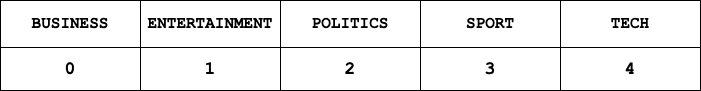
\includegraphics[scale=.5]{./topic_label_relation.png}}
					\caption{mappings between topics and labels}
				\end{figure}
\paragraph{}
Finally, we mapped the five topics to labels ranging from 0 to 4 shown as Figure 1, after which the collection of vectors that represent the given documents can be obtained.

\subsection*{3. Feature Selection, Training and Evaluation}
\subsubsection*{3.1 Feature Selection}
\paragraph{}
Although the top-ranking vocabulary scheme have reduced the potential dimensionality of representation vectors ($30000^+$ without top-ranking selection), we still ended up with a dimensionality of almost 4000. In order to make the dataset less noisy and the model less expensive to train, feature selection is needed. In this regard, we considered the number of selected features $k$ as a hyper-parameter and integrated feature selection process into the pipeline of model training and fine-tuning as following steps: normalisation $\rightarrow$ feature selection $\rightarrow$ training. As for the selection algorithm, we tried both $\chi ^2$ and mutual information schemes, although the selection process ran much faster while using $\chi ^2$ scheme, it's still worth trying both since performance of them have relatively close\cite{3}.
\subsubsection*{3.2. Training and Validation}
\paragraph{}
Our prior knowledge of the given task includes: 
\begin{itemize}
	\item it is a multi-class classification problem; 
	\item sample size is relatively small (only contains 2223 documents); 
	\item dimension of the feature space is high
\end{itemize}
\paragraph{}
From the factors above, both SVM and Softmax Regression could have the capacity to fit well on dataset. To confirm this, we first used a simple train-dev-test(80\%-10\%-10\%) dataset splitting with regular parameter setup to perform a one-shot evaluation (refer to \mintinline{python}{one_shot_eval.py}). If chosen algorithms are underfitting, mis-classification will happen on training set prediction; if algorithms are overfitting, performances on validation set will be poor.
Following code snippets show the evaluation report for both Linear SVM classifier and Softmax Regression, we are therefore confident to say that both methods are capable to perform the task. 
\renewcommand{\thefigure}{2}
\begin{figure}[H]
				\begin{minted}
[frame=lines,
framesep=2mm,
baselinestretch=1.2,
bgcolor=LightGray,
]
{python}
               One-shot test on Softmax Regression
              
   Training Fitting Score:         100.00%
   
   Validation Score:               94.62%
   
   Test Accuracy:                  0.98

                One-shot test on Linear SVM
                    
   Training Fitting Score:         100.00%
   
   Validation Score:               94.62%
   
   Test Accuracy:                  0.96
   
\end{minted}
			\caption{One-shot Validation}
\end{figure}
\paragraph{}
Furthermore, to exploit the dataset and find out which setup of the two algorithms is the best (fine-tuning), we conduct evaluation using Grid Search with 5-fold cross-validation (refer to \mintinline{python}{main.py} and \mintinline{python}{fs_n_train.py}). Started from splitting the whole dataset into training set and test set in 8:2 ratio, we used the training set to perform \mintinline{python}{GridSearchCV} and fine-tune parameters of both algorithms. This will cross-validate each of the hyper-parameter setup we provided %TODO in our case(times of training) 
, and return the predictor which achieved the best overall performance scored by accuracy. Figure 3 and 4 show the cross-validating performance of both algorithms in each parameter grid. As can be seen,
overall performance of Softmax Regression in each parameter setup is more stable than SVM classifier setups, the best setup of Softmax Regression (96.87\%) scored  slightly higher than the best SVM setup (96.47\%) as well.
\renewcommand{\thefigure}{3}
\begin{figure}[H]
				\centerline{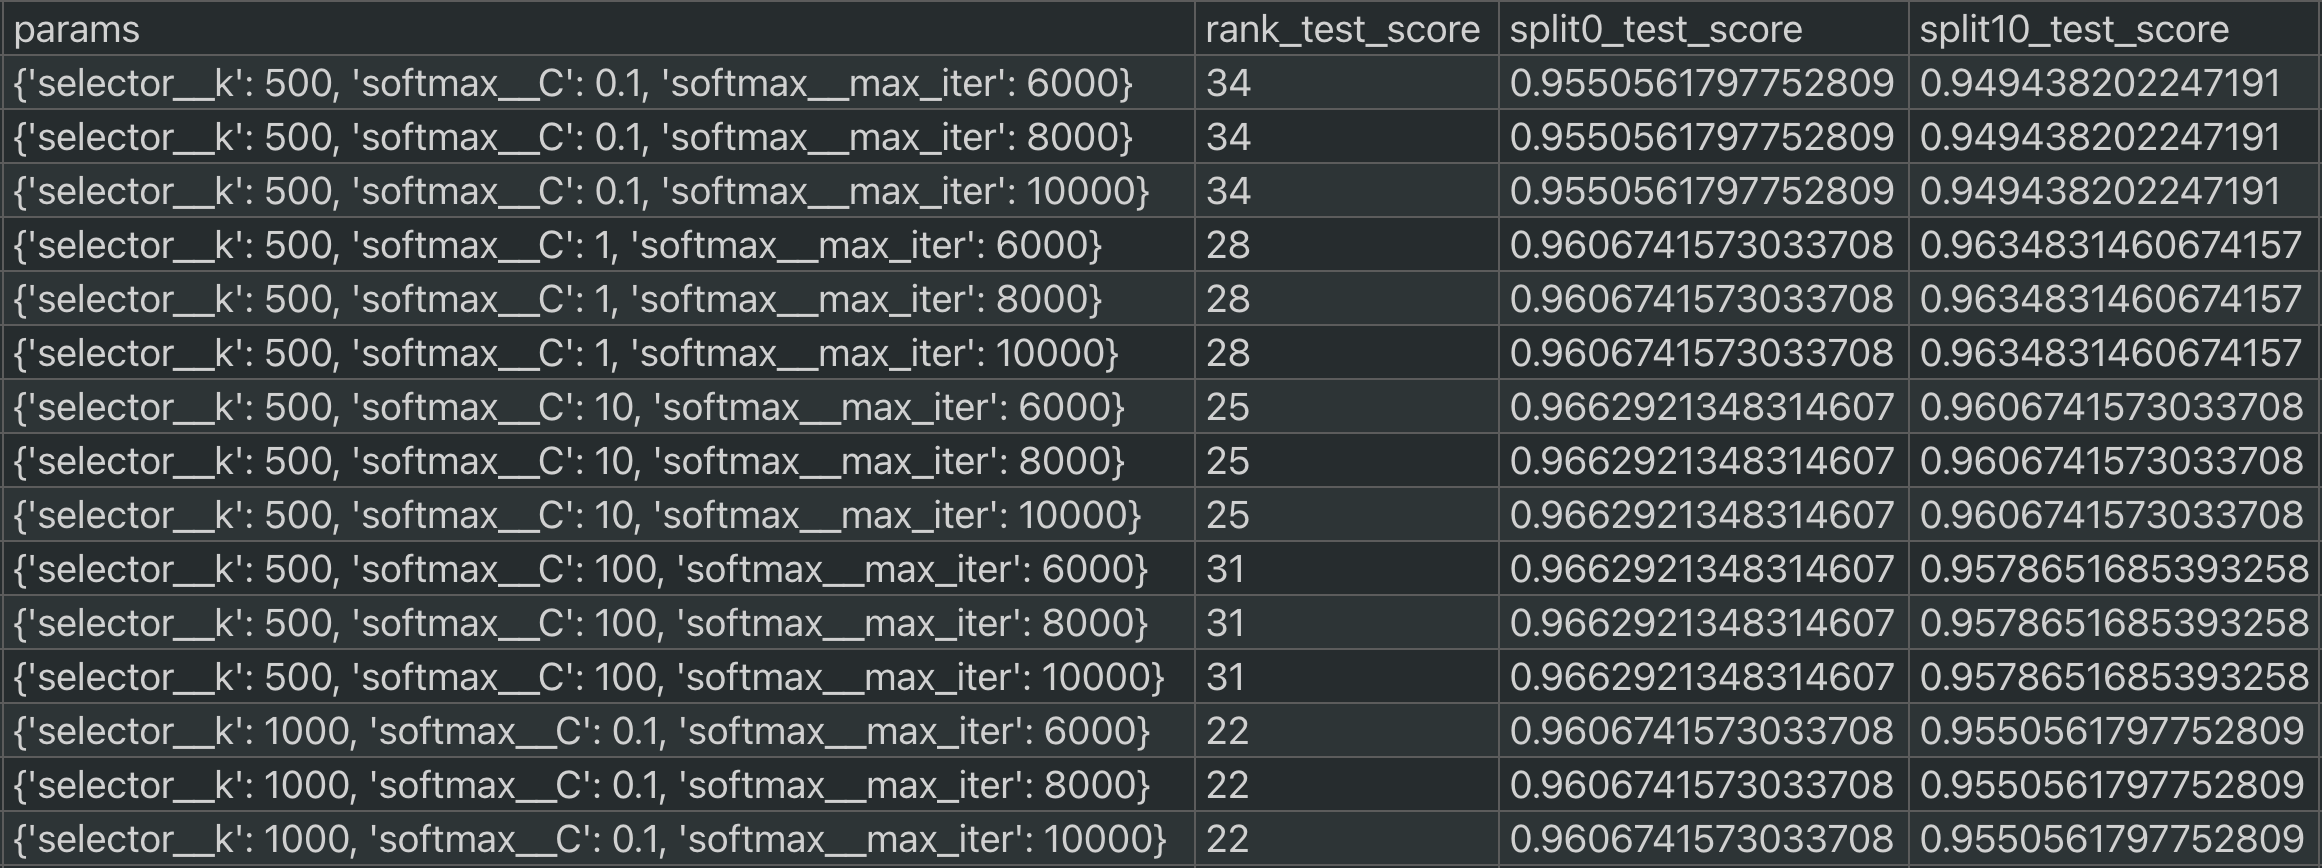
\includegraphics[scale=.3]{./test1_csv.png}}
						\begin{minted}{python}
Score:          96.87%
Parameters: 
{'selector__k': 2000, 'selector__score_func': <function chi2>, 
'softmax__C': 1, 'softmax__max_iter': 5000}
		\end{minted}
					\caption{GridSearchCV Result of Softmax Regression}
\end{figure}
				
\renewcommand{\thefigure}{4}
\begin{figure}[H]
				\centerline{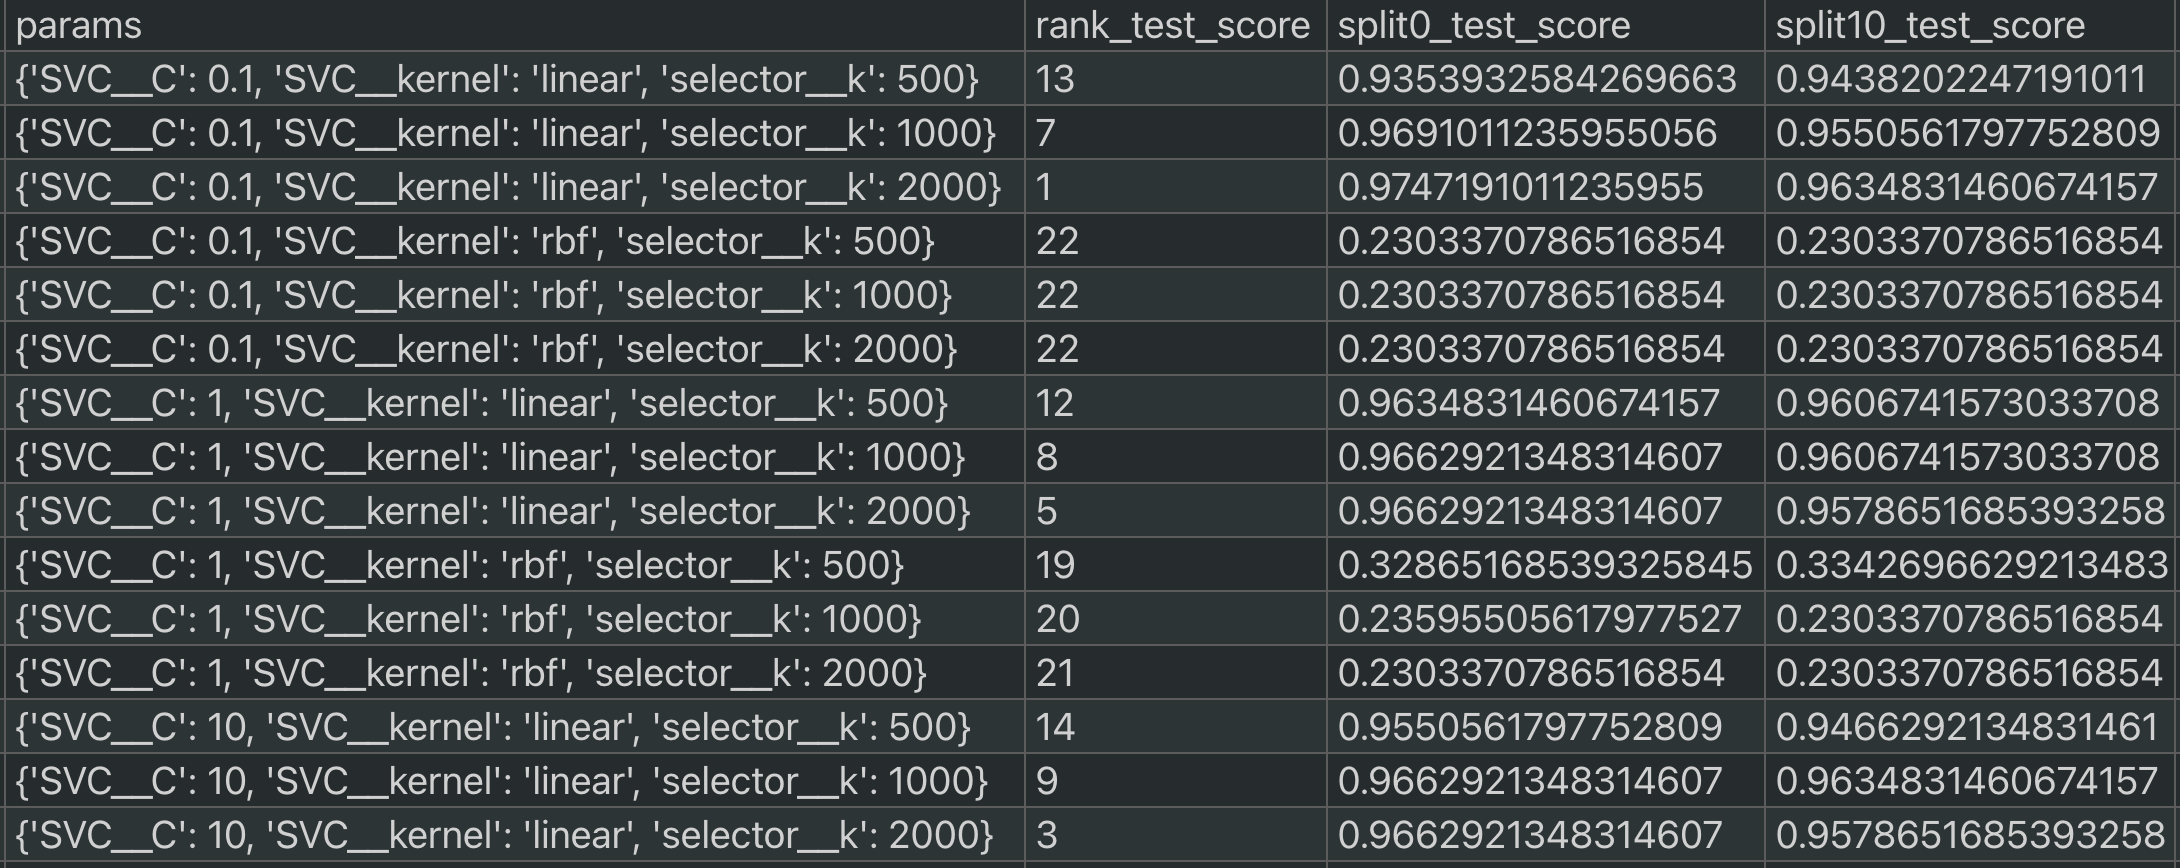
\includegraphics[scale=.3]{./test2_csv.png}}
\begin{minted}{python}
Score:          96.47%
Parameters:	
{'SVC__C': 0.1, 'SVC__kernel': 'linear', 'selector__k': 2000,
'selector__score_func': <function chi2>}
\end{minted}
					\caption{GridSearchCV Result of SVM Classifier}
\end{figure}
 \subsection*{4. Evaluation}
 \paragraph{}
 The next step was using the independently reserved test set to evaluate the performance of chosen best models and give final judgment of chosen models in terms of the unseen data performance, we could be certain that the models generalised dataset well if the result is good. As shown in Figure 5.1.1. to Figure 5.2.2., the best SVC model slightly outperformed the best Softmax Regression model. 
 \paragraph{}
 To test that how well can the models perform beyond the provided dataset, we used them to predict on a small amount of up-to-date unseen test data (refer to \mintinline{python}{unseen_test.py} and, 4 samples for each category), from the confusion matrices shown in Figure 5.3 and Figure 5.4 we can see that SVC model achieved a better performance on the selected unseen data. 
  \renewcommand{\thefigure}{5.1.1.}
		\begin{figure}[H]
				\centerline{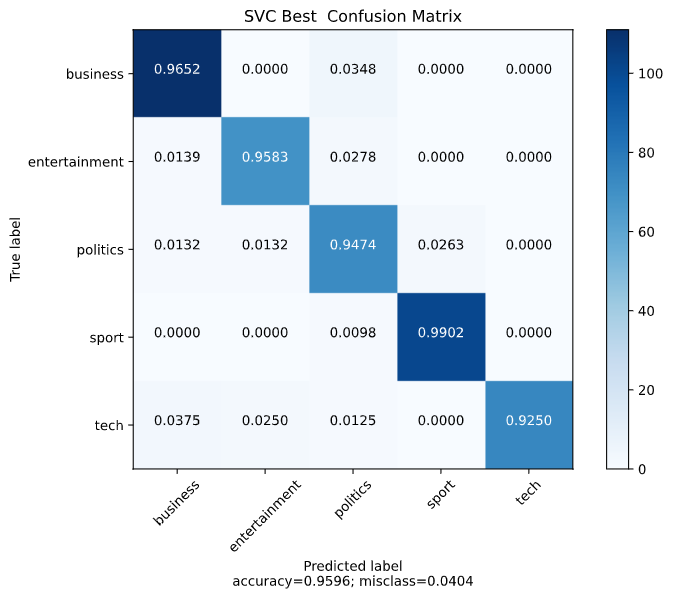
\includegraphics[scale=.4]{./SVC_CM.png}}
					\caption{Confusion Matrix of the best SVC model}
				\end{figure}
\renewcommand{\thefigure}{5.2.2.}
\begin{figure}[H]
				\begin{minted}
[frame=lines,
framesep=2mm,
baselinestretch=1.2,
bgcolor=LightGray,
]
{python}
              precision    recall  f1-score   support

           0       0.96      0.97      0.96       115
           1       0.96      0.96      0.96        72
           2       0.90      0.95      0.92        76
           3       0.98      0.99      0.99       102
           4       1.00      0.93      0.96        80

    accuracy                           0.96       445
   macro avg       0.96      0.96      0.96       445
weighted avg       0.96      0.96      0.96       445

\end{minted}
			\caption{Classification report of the best SVC model}
\end{figure}
				
 \renewcommand{\thefigure}{5.2.1.}
		\begin{figure}[H]
				\centerline{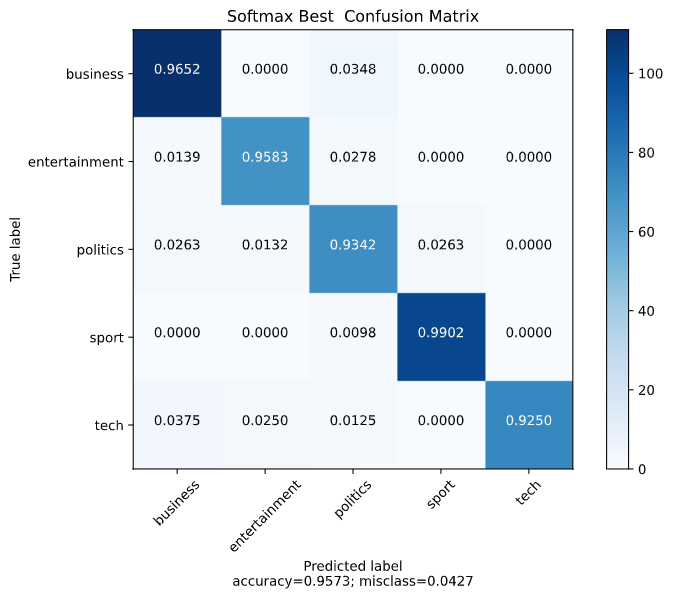
\includegraphics[scale=.4]{./SOFT_CM.png}}
					\caption{Confusion Matrix of the best Softmax Regression model}
				\end{figure}
\renewcommand{\thefigure}{5.1.2.}
\begin{figure}[H]
				\begin{minted}
[frame=lines,
framesep=2mm,
baselinestretch=1.2,
bgcolor=LightGray
]
{python}
              precision    recall  f1-score   support

           0       0.95      0.97      0.96       115
           1       0.96      0.96      0.96        72
           2       0.90      0.93      0.92        76
           3       0.98      0.99      0.99       102
           4       1.00      0.93      0.96        80

    accuracy                           0.96       445
   macro avg       0.96      0.95      0.96       445
weighted avg       0.96      0.96      0.96       445
\end{minted}
			\caption{Classification report of the best Softmax Regression model}
\end{figure}

  \renewcommand{\thefigure}{5.3.}
		\begin{figure}[H]
				\centerline{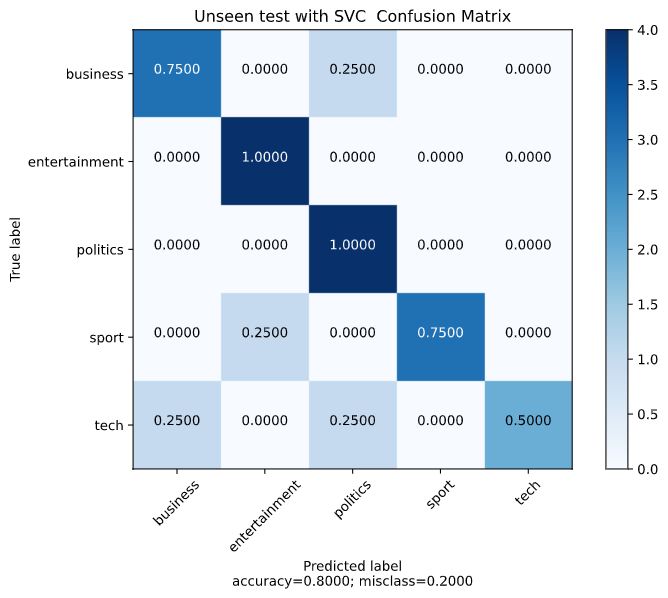
\includegraphics[scale=.4]{./UNSEEN_SVC.png}}
					\caption{Performance of SVC model on unseen data}
				\end{figure}

  \renewcommand{\thefigure}{5.4.}
		\begin{figure}[H]
				\centerline{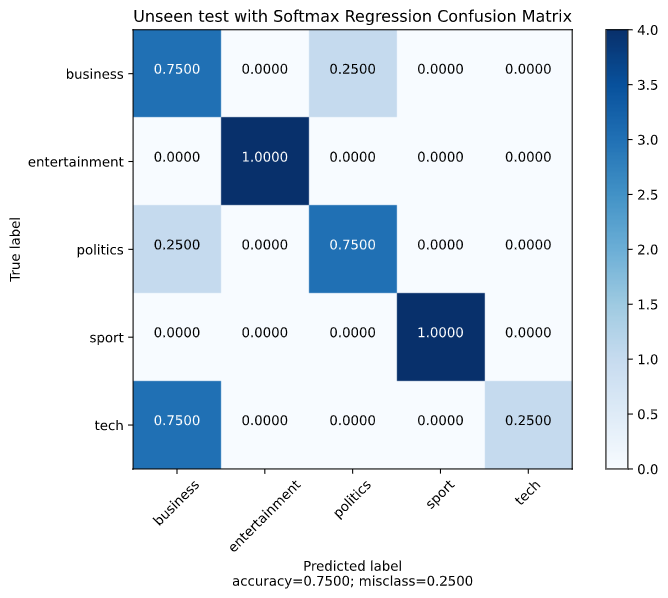
\includegraphics[scale=.4]{./UNSEEN_SOFT.png}}
					\caption{Performance of Softmax Regression model on unseen data}
				\end{figure}


 \subsection*{5. Further Improvements}
 \paragraph{}
 As shown in the predictions of up-to-date data, although our models generalised the dataset well, but when going beyond the dataset, the accuracies significantly dropped. This might due to the following reasons: 
 \begin{enumerate}
 	\item The length of vocabulary in our models are fixed, words that are out-of-vocabulary but relevant to certain topic cannot be identified.
 	\item Our representation approach of documents cannot capture semantics, for instance,  articles which are represented in similar frequency vectors but belong to different topic in actual will be misclassified.
 \end{enumerate}
For improvements, a naive approach is to increase the size of corpus and train the models with new documents, but this could immensely increase the dimensionality of representation and still can do nothing about semantics required factors like synonymy and polysemy. 
 In this case, we can try topic modelling method of representation such as Supervised Latent Dirichlet Allocation\cite{5}., which based on generative model and has greater capacities in text representation and semantics capturing .(See section 6 for more details)
 
 \subsection*{6. Literature Review of sLDA(Optional)}
 \paragraph{}
 \textit{Supervised Latent Dirichlet allocation}(sLDA) is a derivation of
 \textit{Latent Dirichlet allocation} (LDA), a generative probabilistic topic modelling approach for discovering "topics" that occur in a collection of documents. 
 The basic ideas of LDA are modelling the documents in a collection as a mixture over an underlying set of topics, and the set of topics are modelled as probability distributions over words in documents\cite{5}. While LDA is an unsupervised approach, sLDA provides a supervised topic model, where each document is paired with a response. After topic model is built, sLDA can be used to infer the topic structure of an unlabelled document\cite{6}.
 \paragraph{}
 Here we illustrate the power of topics modelling by a simple test case (refer to \mintinline{python}{sLDA_test.py}).
 When training the news classifier with sLDA representation, the dimensionality of representation vectors reduced significantly comparing to \textit{bag of words} approach(from almost 4000 to only 5). Also, as shown in Figure 6.1 and Figure 6.2, although the untuned model has a slightly lower accuracy than our previous best fine-tuned model, but it performed incredibly well on the up-to-date unseen samples, which can somehow show that topic modelling approach is more flexible and robust than BoW.
 \renewcommand{\thefigure}{6.1.}
\begin{figure}[H]
				\begin{minted}
[frame=lines,
framesep=2mm,
baselinestretch=1.2,
bgcolor=LightGray
]
{python}
              precision    recall  f1-score   support

           0       0.92      0.90      0.91        40
           1       1.00      0.88      0.94        42
           2       0.91      0.93      0.92        42
           3       0.98      1.00      0.99        57
           4       0.87      0.95      0.91        41

    accuracy                           0.94       222
   macro avg       0.94      0.93      0.93       222
weighted avg       0.94      0.94      0.94       222
\end{minted}

\centerline{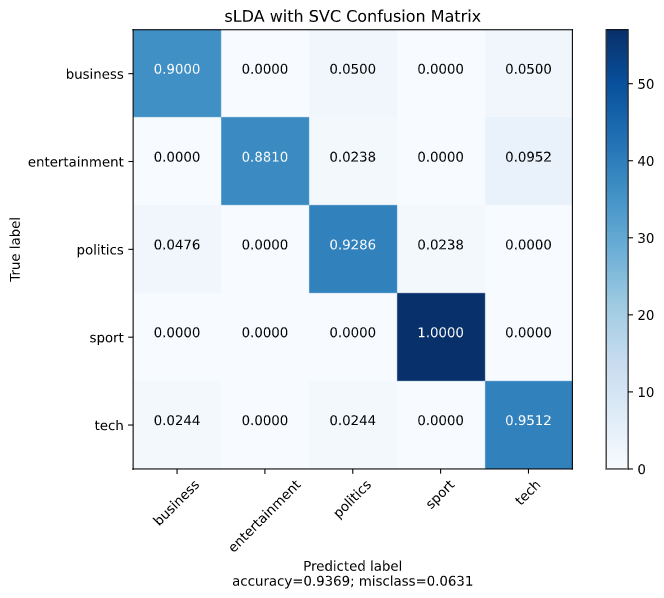
\includegraphics[scale=.4]{./sLDA_test_cm.png}}
			\caption{Classification report of sLDA modelling with linear SVC}
\end{figure}

 \renewcommand{\thefigure}{6.2.}
\begin{figure}[H]
				\begin{minted}
[frame=lines,
framesep=2mm,
baselinestretch=1.2,
bgcolor=LightGray
]
{python}
              precision    recall  f1-score   support

           0       0.80      1.00      0.89         4
           1       1.00      1.00      1.00         4
           2       0.80      1.00      0.89         4
           3       1.00      1.00      1.00         4
           4       1.00      0.50      0.67         4

    accuracy                           0.90        20
   macro avg       0.92      0.90      0.89        20
weighted avg       0.92      0.90      0.89        20
\end{minted}

\centerline{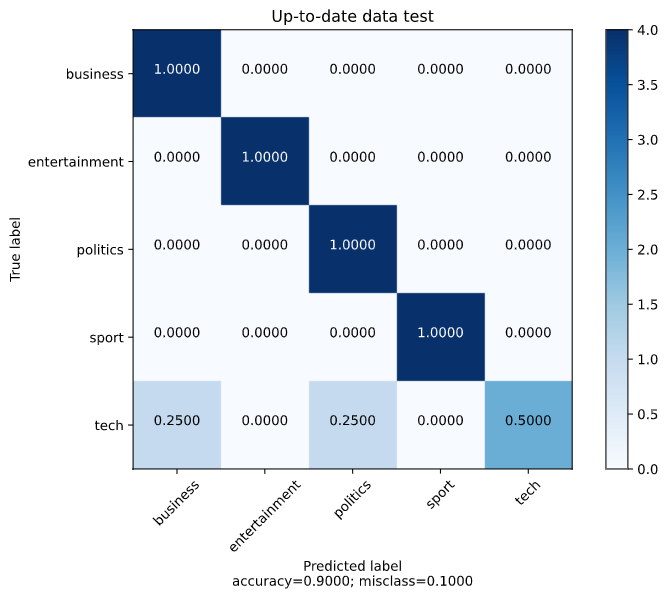
\includegraphics[scale=.4]{./sLDA_utd_test_cm.png}}
			\caption{Classification report of sLDA modelling with linear SVC}
\end{figure}
\clearpage
 
\begin{thebibliography}{9}
\bibitem{ml_in_atc} 
Fabrizio Sebastiani. 
\textit{Machine learning in Automated Text Categorization}. 
\textit{ACM Computing Surveys}, March 2002 
\\\texttt{https://dl.acm.org/doi/pdf/10.1145/505282.505283}

\bibitem{iir} 
Christopher D. Manning, Prabhakar Raghavan and Hinrich Schütze. 
\textit{Introduction to Information Retrieval}.
Cambridge University Press, ISBN 0521865719. 2008.
\\\texttt{https://nlp.stanford.edu/IR-book/}

\bibitem{iir2} 
Christopher D. Manning, Prabhakar Raghavan and Hinrich Schütze. 
\textit{Introduction to Information Retrieval: Comparison of feature selection methods}.
Cambridge University Press, ISBN 0521865719. 2008.
\\\texttt{https://nlp.stanford.edu/IR-book/html/htmledition/
\\
comparison-of-feature-selection-methods-1.html}

\bibitem{ds}
D. Greene and P. Cunningham. \textit{"Practical Solutions to the Problem of Diagonal Dominance in Kernel Document Clustering"}, Proc. ICML 2006.

\bibitem{lda}
D. M. Blei, ‘\textit{Latent Dirichlet Allocation}’, p. 30.


\bibitem{slda}
J. D. Mcauliffe and D. M. Blei, ‘\textit{Supervised Topic Models}’, p. 8.



\end{thebibliography}

\medskip

\end{document}